\documentclass[10pt,a4paper]{article}
\usepackage[margin=22mm]{geometry}
\usepackage[T1]{fontenc}
\usepackage{lmodern,amsmath,amssymb,booktabs,graphicx,tikz,hyperref,fvextra}
\usetikzlibrary{arrows.meta,positioning,calc,decorations.pathmorphing}
\definecolor{ink}{RGB}{20,53,78}
\hypersetup{colorlinks=true,urlcolor=ink,linkcolor=ink}
\setlength{\parindent}{0pt}
\setlength{\parskip}{5pt}
\emergencystretch=3em

\title{\color{ink}Sampling can destabilize a continuous-time design}
\author{}
\date{Original learning collection -- November 2026}
\begin{document}
\begin{center}{\LARGE\color{ink}Sampling can destabilize a continuous-time design}\\[5pt]{\small Original learning collection -- November 2026}\end{center}

\textbf{Evidence note.} Original teaching scenario. Numerical parameters are deliberately chosen for learning. All generated data and curves are synthetic; no physical measurement is asserted.
\section{Design brief}
For $G(s)=1/(0.5s+1)$, use PI gains $k_p=2$ and $k_i=4$ with a held actuator. Apply $u_k=2(r_k-x_k)+I_k$ before updating $I_{k+1}=I_k+4T_s(r_k-x_k)$. Derive the exact sampled plant update and two-state closed-loop matrix. Compare $T_s=0.05$, $0.5$ and $1.0\,\mathrm{s}$ and find the first discrete-time stability boundary.
\section{Physical system}
\begin{center}\resizebox{\ifdim\width>.98\linewidth.98\linewidth\else\width\fi}{!}{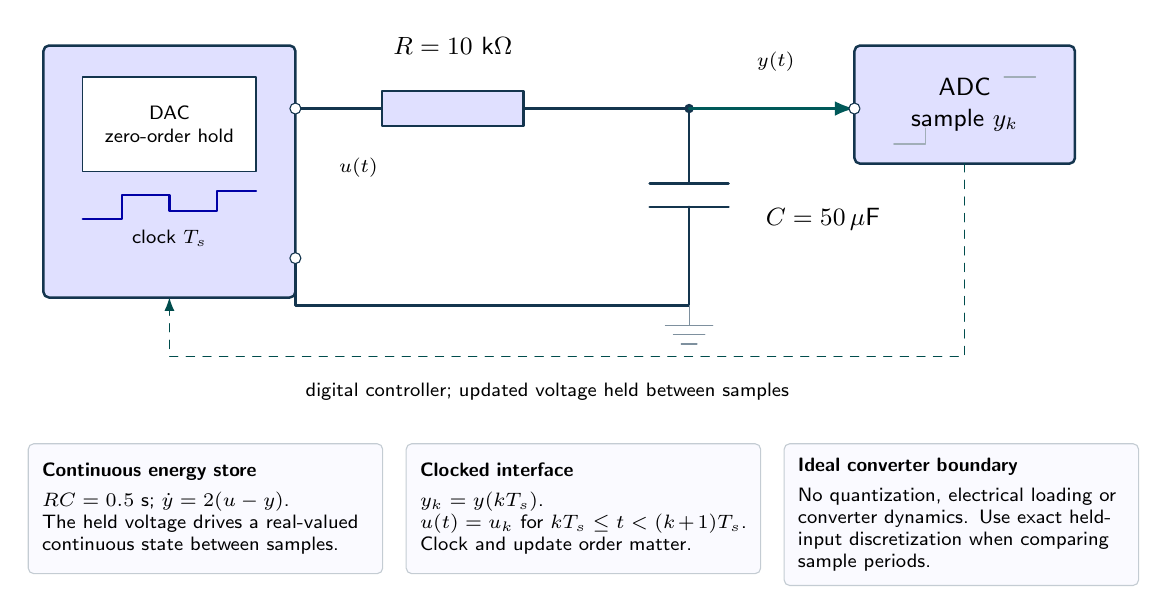
\begin{tikzpicture}[
font=\sffamily\small,>=Latex,line cap=round,line join=round,
wall/.style={draw=ink,line width=1.2pt,fill=blue!5},
water/.style={fill=cyan!25,draw=none},
metal/.style={draw=ink,fill=blue!12,line width=.9pt},
flow/.style={->,draw=blue!65!black,line width=1.2pt},
heat/.style={->,draw=orange!85!black,line width=1.1pt},
measure/.style={->,draw=teal!70!black,line width=.9pt},
dim/.style={<->,draw=ink!65,line width=.6pt},
spring/.style={draw=ink,decorate,decoration={coil,aspect=.5,segment length=4pt,amplitude=3pt}},
wire/.style={draw=ink,line width=1pt},
lab/.style={align=center,font=\sffamily\small},
smalllab/.style={align=center,font=\sffamily\scriptsize}]

\draw[metal,rounded corners=2pt](.2,1)rectangle(3.4,4.2);
\draw[fill=white,draw=ink](.7,2.6)rectangle(2.9,3.8);
\node[smalllab]at(1.8,3.2){DAC\\zero-order hold};
\node[smalllab]at(1.8,1.75){clock $T_s$};
\draw[wire](3.4,3.4)--(4.5,3.4);
\draw[metal](4.5,3.18)rectangle(6.3,3.62);
\draw[wire](6.3,3.4)--(8.4,3.4)--(8.4,2.45);
\draw[wire](7.9,2.45)--(8.9,2.45)(7.9,2.15)--(8.9,2.15);
\draw[wire](8.4,2.15)--(8.4,.9)--(3.4,.9)--(3.4,1.5);
\node[lab]at(5.4,4.2){$R=10$ k$\Omega$};
\node[lab,anchor=west]at(9.25,2.0){$C=50\,\mu$F};
\fill[ink](8.4,3.4)circle(.06);
\draw[measure](8.4,3.4)--(10.5,3.4);
\draw[metal,rounded corners=2pt](10.5,2.7)rectangle(13.3,4.2);
\node[lab]at(11.9,3.45){ADC\\sample $y_k$};
\draw[teal!60!black,dashed,->](11.9,2.7)--(11.9,.25)--(1.8,.25)--(1.8,1);
\node[smalllab]at(6.6,-.2){digital controller; updated voltage held between samples};
\node[smalllab]at(4.2,2.65){$u(t)$};
\node[smalllab]at(9.5,4){$y(t)$};
% REFINED EQUIPMENT DETAILS

% Held waveform, converter terminals and common electrical reference.
\draw[blue!65!black,line width=.8pt](.7,2)--(1.2,2)--(1.2,2.3)--(1.8,2.3)--(1.8,2.1)--(2.4,2.1)--(2.4,2.35)--(2.9,2.35);
\foreach \x/\y in {3.4/3.4,3.4/1.5,10.5/3.4}{\draw[ink,fill=white](\x,\y)circle(.07);}
\draw[ink!55](8.4,.9)--(8.4,.65)(8.1,.65)--(8.7,.65)(8.2,.53)--(8.6,.53)(8.3,.41)--(8.5,.41);
\draw[ink!40](11,2.95)--(11.4,2.95)--(11.4,3.15)(12.4,3.8)--(12.8,3.8);

\node[draw=ink!25,fill=blue!2,rounded corners=2pt,anchor=north west,text width=4.15cm,minimum height=1.65cm,inner sep=5pt,align=left,font=\sffamily\scriptsize]at(0.0,-0.85){\textbf{Continuous energy store}\\[3pt]$RC=0.5$ s; $\dot y=2(u-y)$.\\The held voltage drives a real-valued continuous state between samples.};
\node[draw=ink!25,fill=blue!2,rounded corners=2pt,anchor=north west,text width=4.15cm,minimum height=1.65cm,inner sep=5pt,align=left,font=\sffamily\scriptsize]at(4.8,-0.85){\textbf{Clocked interface}\\[3pt]$y_k=y(kT_s)$.\\$u(t)=u_k$ for $kT_s\leq t<(k+1)T_s$.\\Clock and update order matter.};
\node[draw=ink!25,fill=blue!2,rounded corners=2pt,anchor=north west,text width=4.15cm,minimum height=1.65cm,inner sep=5pt,align=left,font=\sffamily\scriptsize]at(9.6,-0.85){\textbf{Ideal converter boundary}\\[3pt]No quantization, electrical loading or converter dynamics. Use exact held-input discretization when comparing sample periods.};
\end{tikzpicture}
}\par{\small A held voltage drives an ideal RC network. The capacitor voltage is sampled by an ideal ADC; the software controller updates the DAC once per period. Quantization, converter lag and electrical loading are omitted.}\end{center}
\section{Continuous design}
The continuous PI characteristic polynomial is $0.5s^2+3s+4=0.5(s+2)(s+4)$, so its poles are stable. This does not establish the stability of a particular digital implementation.
\section{Exact held-input plant}
Holding $u[k]$ over one sample interval gives $x[k+1]=ax[k]+bu[k]$, where $a=e^{-2T_s}$ and $b=1-a$. The explicit integral update uses the old sample error, so for zero reference,
\[\begin{bmatrix}x[k+1]\\I[k+1]\end{bmatrix}=M(T_s)\begin{bmatrix}x[k]\\I[k]\end{bmatrix},\quad
M=\begin{bmatrix}a-2b&b\\-4T_s&1\end{bmatrix}.\]
Changing the order of integral update and actuator computation would change this matrix.
\section{Unit-circle test}
Discrete stability requires every eigenvalue of $M$ to lie strictly inside the unit circle. With trace $t=3a-1$ and determinant $d=3a-2+4T_s(1-a)$, the second-order Jury conditions are $1-t+d>0$, $1+t+d>0$, and $1-d>0$.
For $T_s>0$, the first expression is $4T_s(1-a)>0$. The determinant becomes one at $T_s=0.75$ s, where the conjugate pair lies on the unit circle. The remaining conditions hold up to that crossing. Thus the first stable interval is $0<T_s<0.75$ s, and the endpoint is excluded.
\section{Evidence and limits}
Plot samples explicitly rather than connecting them as if they were continuous measurements. These results assume exact model parameters, an instantaneous computation at each sample, and no extra communication delay or actuator saturation.
\section{What to learn from the experiment}
A stable continuous controller can fail after discretization. State the sampling rule and update order, then test the actual discrete closed-loop model.
\section{System sketch}
\begin{center}\resizebox{\ifdim\width>.98\linewidth.98\linewidth\else\width\fi}{!}{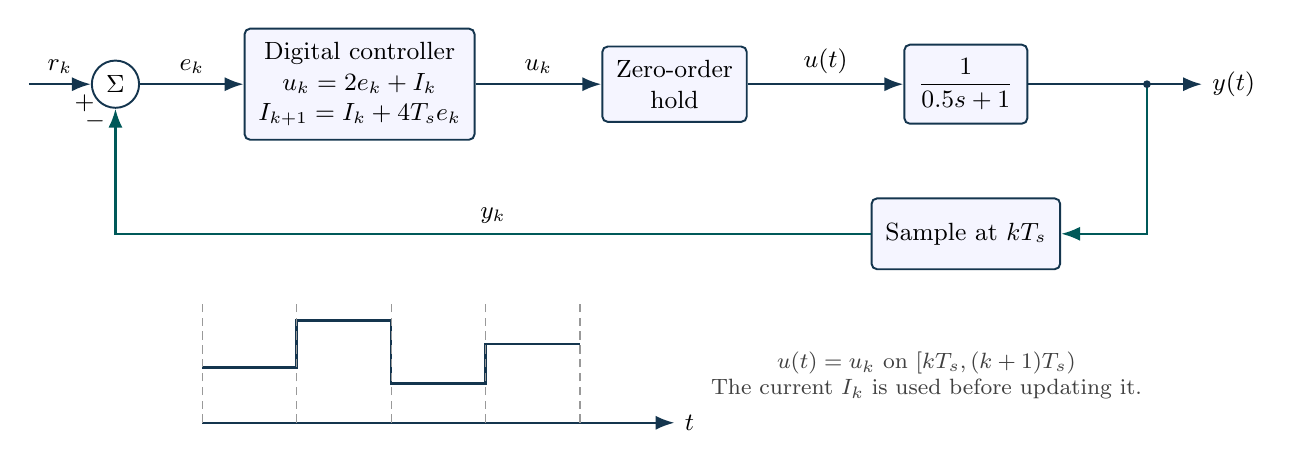
\begin{tikzpicture}[x=1cm,y=1cm,>=Latex,font=\small,
block/.style={draw=ink,fill=blue!4,rounded corners=2pt,minimum height=9mm,align=center,line width=.7pt,inner sep=5pt},
sum/.style={circle,draw=ink,fill=white,minimum size=6mm,inner sep=0pt,line width=.7pt},
sig/.style={->,draw=ink,line width=.85pt},
fb/.style={->,draw=teal!70!black,line width=.85pt},
dist/.style={->,draw=orange!75!black,line width=.85pt},
tap/.style={circle,fill=ink,inner sep=1.4pt},
note/.style={font=\footnotesize,align=center,text=black!75}]

\node[sum](e)at(.9,1.5){$\Sigma$};
\node[block,minimum height=14mm](c)at(4,1.5){Digital controller\\$u_k=2e_k+I_k$\\$I_{k+1}=I_k+4T_se_k$};
\node[block](zoh)at(8,1.5){Zero-order\\hold};
\node[block](p)at(11.7,1.5){$\dfrac{1}{0.5s+1}$};
\draw[sig](-.2,1.5)--node[above]{$r_k$}node[pos=.9,below]{$+$}(e);
\draw[sig](e)--node[above]{$e_k$}(c);
\draw[sig](c)--node[above]{$u_k$}(zoh);
\draw[sig](zoh)--node[above]{$u(t)$}(p);
\draw[sig](p)--(14.7,1.5)node[right]{$y(t)$};
\node[block](sam)at(11.7,-.4){Sample at $kT_s$};
\draw[fb](14,1.5)--(14,-.4)--(sam);
\fill[ink](14,1.5)circle(1.4pt);
\draw[fb](sam)--node[above]{$y_k$}(.9,-.4)--node[pos=.9,left]{$-$}(e);
\draw[sig](2,-2.8)--(8,-2.8)node[right]{$t$};
\draw[line width=1pt,draw=ink](2,-2.1)--(3.2,-2.1)--(3.2,-1.5)--(4.4,-1.5)--(4.4,-2.3)--(5.6,-2.3)--(5.6,-1.8)--(6.8,-1.8);
\foreach \x in{2,3.2,4.4,5.6,6.8}{\draw[black!40,densely dashed](\x,-2.8)--(\x,-1.25);}
\node[note]at(11.2,-2.2){$u(t)=u_k$ on $[kT_s,(k+1)T_s)$\\The current $I_k$ is used before updating it.};

\end{tikzpicture}
}
\par\small\refstepcounter{figure}\label{fig:system}\textbf{Figure \thefigure.} The sampler, digital update order and hold are explicit. Continuous plant dynamics and sampled controller states occupy different parts of the loop.\end{center}
\section{Executed computational evidence}
\VerbatimInput[fontsize=\small,breaklines=true]{results.txt}
\begin{center}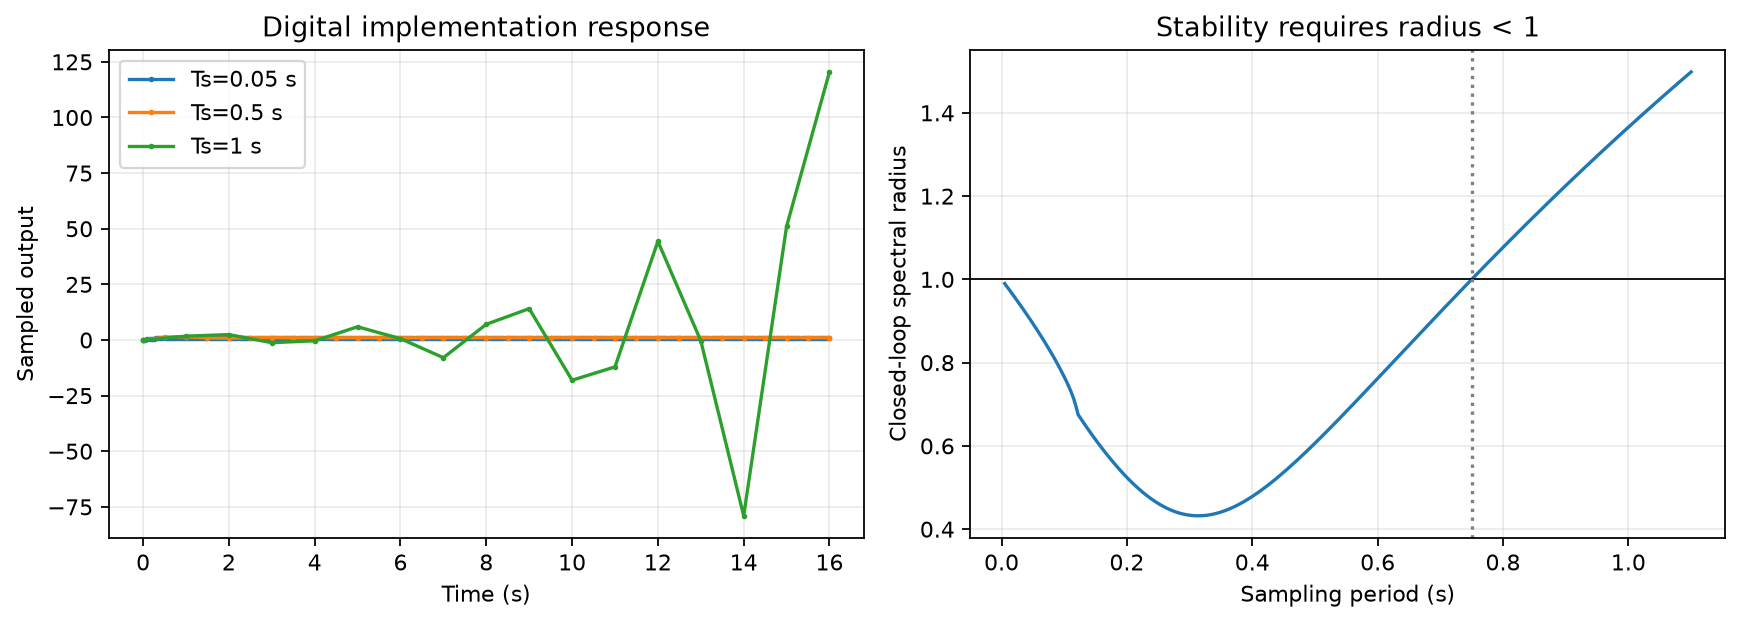
\includegraphics[width=\linewidth,height=.16\textheight,keepaspectratio]{response.png}\end{center}
\paragraph{Method references.}
The equations use standard balance laws and feedback-control methods. Further explanation: \url{https://apmonitor.com/pdc/} and \url{https://fbsbook.org/}. Implementation documentation: \url{https://python-control.readthedocs.io/en/0.10.2/}. See the repository reference catalog for individual topics and videos.
\end{document}
